\subsection{実験結果}
\label{sec_results}

選定した UFB 濃度，MB 濃度，酸素含量の 3 つの目的変数それぞれについて，説明変数から目的変数を予測する回帰モデルとして，線形回帰，多項式回帰，Random Forest の 3 種類を学習した．
線形回帰は 6 つの説明変数に対する線形結合により目的変数を予測するモデルであり，多項式回帰は各説明変数の 2 次の項および交互作用項まで拡張した上で線形回帰を適用するモデルである．
Random Forest は，学習データから復元抽出したサブサンプルおよび分岐候補となる説明変数をランダムに選択して構築した複数の決定木の予測値を平均する回帰モデルであり，本研究では決定木数を 100，各決定木の最大深さを 5 に設定した．

モデルの評価には，同一操作条件のサンプルが学習用データと評価用データに分かれて混入しないよう，操作条件を単位としてグループ化した 5-fold の Group $ k $-分割交差検証を用いた．
各モデルの予測誤差の指標には，式(\ref{eq_rmse})に示す平均二乗誤差平方根（Root Mean Squared Error，RMSE）を用いた．

\begin{equation}
    \mathrm{RMSE} = \sqrt{ \frac{1}{N} \sum_{i=1}^{N} \left( z_i - \hat{z}_i \right)^2 }
    \label{eq_rmse}
\end{equation}

\noindent
ここで $ z_i $ は標準化後の目的変数の真値，$ \hat{z}_i $ はモデルによる予測値，$ N $ はサンプル数である．
目的変数を標準化した上で RMSE を算出しているため，異なる目的変数間でも予測誤差の大きさを比較できる．

表\ref{tab_rmse}に，3 つの目的変数それぞれについて学習用データ（Train）および評価用データ（Test）に対する RMSE を示す．
いずれの目的変数についても Random Forest が最も低い Test RMSE を示し，3 つのモデルの中で最も高い予測性能を示した．
特に，多項式回帰は UFB 濃度において Train RMSE（$ 0.695 $）に対して Test RMSE（$ 1.168 $）が大きく上回っており，モデルが学習データに過剰適合している．
これは，6 つの説明変数を 2 次まで拡張したことでモデルのパラメータ数がサンプル数（82 サンプル）に対して相対的に多くなり，過学習が生じやすくなったためと考えられる．
一方，Random Forest は決定木の最大深さを制限した上で複数の決定木の予測を平均するため，Train RMSE と Test RMSE の乖離が 3 つのモデルの中で最も小さく，過学習が抑制されていることが確認できる．

\begin{table}[H]
    \caption{3 種のモデルによる目的変数ごとの Train／Test RMSE}
    \centering
    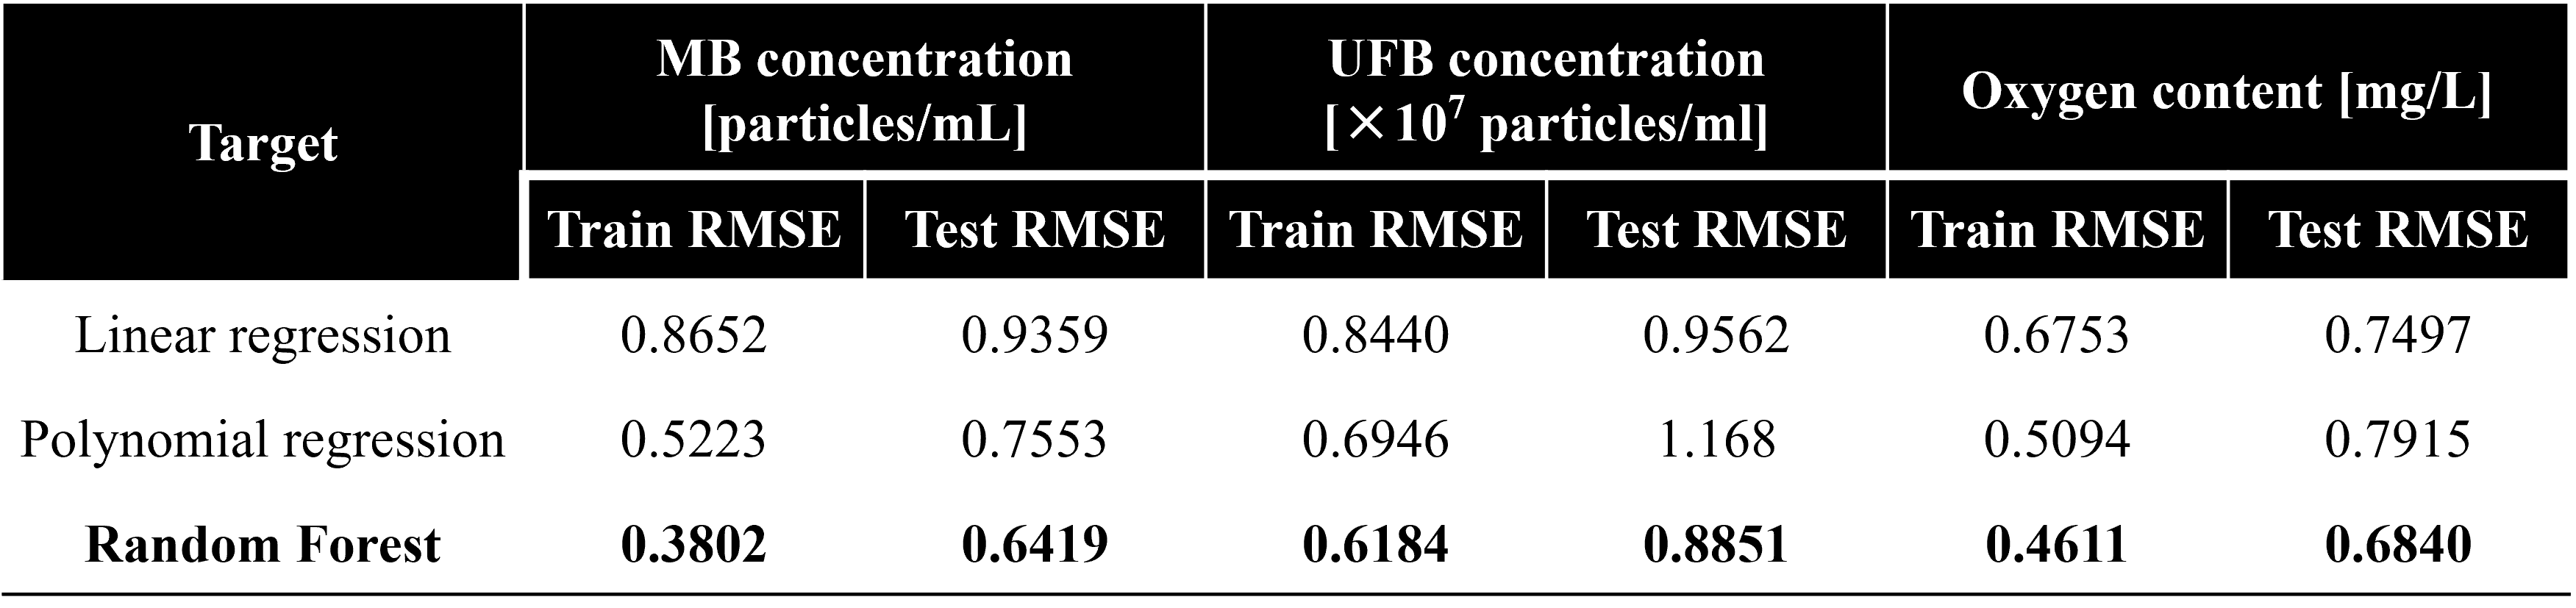
\includegraphics[width=\linewidth]{figures/table2_training_result.png}
    \label{tab_rmse}
\end{table}

Random Forest がどの説明変数を重視して予測を行っているかを分析するため，Mean Decrease in Impurity（MDI）に基づく Feature Importance を算出した．
本研究は回帰問題であるため，Feature Importance は式(\ref{eq_fi})に示す通り，森を構成する各決定木において，説明変数 $ j $ による分岐がもたらす二乗誤差の減少量を，その分岐に到達したサンプルの割合で重み付けして合計し，決定木数で平均した値として定義した．

\begin{equation}
    \mathrm{FI}_j = \frac{1}{T} \sum_{t=1}^{T} \sum_{v \in V_{t,j}} \frac{ n_v }{ n } \Delta e_v
    \label{eq_fi}
\end{equation}

\noindent
ここで $ T $ は決定木数，$ V_{t,j} $ は決定木 $ t $ において説明変数 $ j $ で分岐しているノードの集合，$ n_v $ はノード $ v $ に到達したサンプル数，$ n $ は全サンプル数，$ \Delta e_v $ はノード $ v $ における分岐前後の二乗誤差の減少量である．
本研究では，交差検証の各 fold で学習した Random Forest の Feature Importance を fold 間で平均した値を用いた．

図\ref{fig_fi} に，MB 濃度，UFB 濃度，酸素含量それぞれに対する Feature Importance を示す．

\begin{figure}[H]
    \centering
    \begin{subfigure}[b]{0.32\linewidth}
        \centering
        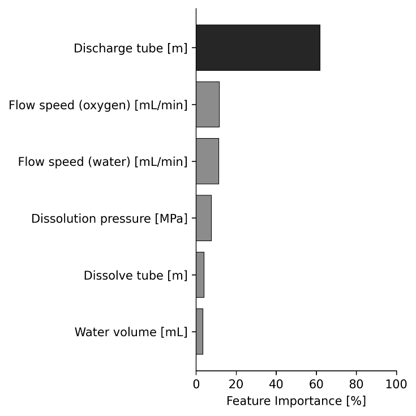
\includegraphics[width=\linewidth]{figures/figure3A_MB_feature_importance.png}
        \caption{MB 濃度}
        \label{fig_fi_mb}
    \end{subfigure}
    \hfill
    \begin{subfigure}[b]{0.32\linewidth}
        \centering
        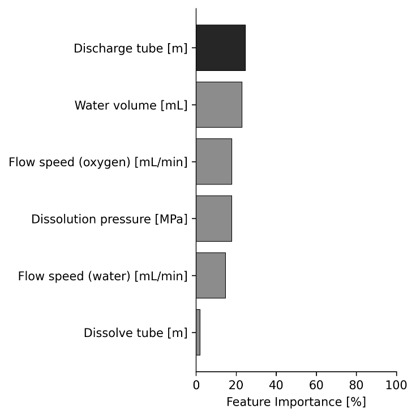
\includegraphics[width=\linewidth]{figures/figure3B_UFB_feature_importance.png}
        \caption{UFB 濃度}
        \label{fig_fi_ufb}
    \end{subfigure}
    \hfill
    \begin{subfigure}[b]{0.32\linewidth}
        \centering
        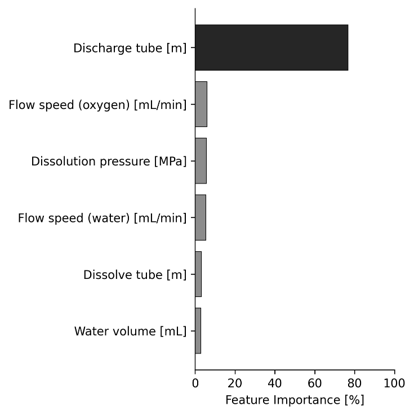
\includegraphics[width=\linewidth]{figures/figure3C_Oxygen_feature_importance.png}
        \caption{酸素含量}
        \label{fig_fi_oxygen}
    \end{subfigure}
    \par\vspace{2mm}
    \caption{目的変数ごとの Feature Importance}
    \label{fig_fi}
\end{figure}

図\ref{fig_fi}(A)および図\ref{fig_fi}(C)から，MB 濃度および酸素含量では，いずれも Discharge tube の Feature Importance が突出して高く（それぞれ約 $ 62\,\% $，約 $ 77\,\% $），単一の説明変数が支配的な重要度を示していることがわかる．
一方，図\ref{fig_fi}(B)から，UFB 濃度では Discharge tube が最も高い重要度を示すものの，Water volume，Flow speed (oxygen)，Dissolution pressure の重要度も同程度の水準にあり，特定の説明変数に支配されない分散した重要度分布となっていることがわかる．

3 つの目的変数のいずれにおいても Feature Importance が最大であった Discharge tube について，各水準における目的変数の分布を図\ref{fig_box}に箱ひげ図として示す．

\begin{figure}[H]
    \centering
    \begin{subfigure}[b]{0.32\linewidth}
        \centering
        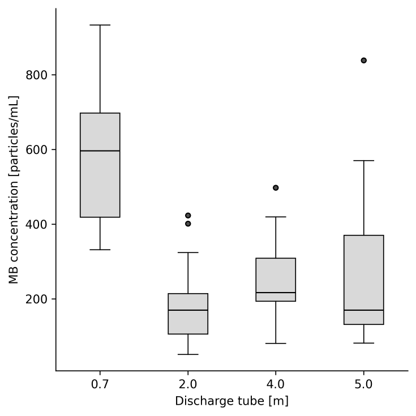
\includegraphics[width=\linewidth]{figures/figure4A_MB_box_plot.png}
        \caption{MB 濃度}
        \label{fig_box_mb}
    \end{subfigure}
    \hfill
    \begin{subfigure}[b]{0.32\linewidth}
        \centering
        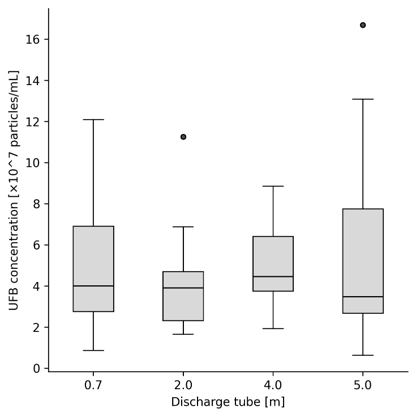
\includegraphics[width=\linewidth]{figures/figure4B_UFB_box_plot.png}
        \caption{UFB 濃度}
        \label{fig_box_ufb}
    \end{subfigure}
    \hfill
    \begin{subfigure}[b]{0.32\linewidth}
        \centering
        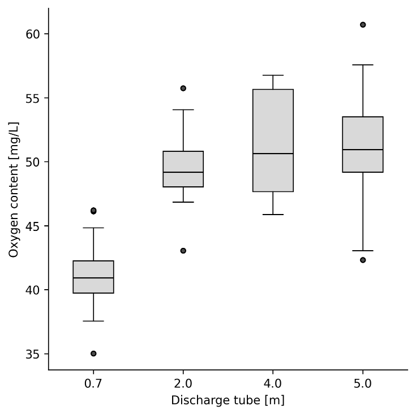
\includegraphics[width=\linewidth]{figures/figure4C_Oxygen_box_plot.png}
        \caption{酸素含量}
        \label{fig_box_oxygen}
    \end{subfigure}
    \par\vspace{2mm}
    \caption{Discharge tube と目的変数の関係}
    \label{fig_box}
\end{figure}

図\ref{fig_box}(A)から，MB 濃度は Discharge tube が $ 0.7\,\mathrm{m} $ で中央値が最も高く（約 $ 595 $），$ 2.0\,\mathrm{m} $ で最も低くなった後，$ 4.0\,\mathrm{m} $，$ 5.0\,\mathrm{m} $ にかけて分布が再び広がる非単調な関係を示すことがわかる．
図\ref{fig_box}(B)から，UFB 濃度は Discharge tube の各水準で中央値に明確な単調傾向はみられず，特に $ 5.0\,\mathrm{m} $ において分布の広がりが大きくなることがわかる．
図\ref{fig_box}(C)から，酸素含量は Discharge tube が長くなるにつれて中央値が単調に上昇する傾向を示す（$ 0.7\,\mathrm{m} $ で約 $ 41\,\mathrm{mg/L} $，$ 5.0\,\mathrm{m} $ で約 $ 51\,\mathrm{mg/L} $）ことがわかる．
